%%%%%%%%%%%%%%%%%%%%%%%%%%%%%%%%%%%%%%%%%
% Thin Sectioned Essay
% LaTeX Template
% Version 1.0 (3/8/13)
%
% This template has been downloaded from:
% http://www.LaTeXTemplates.com
%
% Original Author:
% Nicolas Diaz (nsdiaz@uc.cl) with extensive modifications by:
% Vel (vel@latextemplates.com)
%
% License:
% CC BY-NC-SA 3.0 (http://creativecommons.org/licenses/by-nc-sa/3.0/)
%
%%%%%%%%%%%%%%%%%%%%%%%%%%%%%%%%%%%%%%%%%

%----------------------------------------------------------------------------------------
%	PACKAGES AND OTHER DOCUMENT CONFIGURATIONS
%----------------------------------------------------------------------------------------

\documentclass[a4paper, 11pt]{article} % Font size (can be 10pt, 11pt or 12pt) and paper size (remove a4paper for US letter paper)

\usepackage[protrusion=true,expansion=true]{microtype} % Better typography
\usepackage{graphicx} % Required for including pictures
\graphicspath{{images/}}
\usepackage{wrapfig} % Allows in-line images

\usepackage{amsmath} 
\usepackage{mathpazo} % Use the Palatino font
\usepackage[T1]{fontenc} % Required for accented characters
\linespread{1.05} % Change line spacing here, Palatino benefits from a slight increase by default

\makeatletter
\renewcommand\@biblabel[1]{\textbf{#1.}} % Change the square brackets for each bibliography item from '[1]' to '1.'
\renewcommand{\@listI}{\itemsep=0pt} % Reduce the space between items in the itemize and enumerate environments and the bibliography

\renewcommand{\maketitle}{ % Customize the title - do not edit title and author name here, see the TITLE block below
\begin{flushright} % Right align
{\LARGE\@title} % Increase the font size of the title

\vspace{50pt} % Some vertical space between the title and author name

{\large\@author} % Author name
\\\@date % Date

\vspace{40pt} % Some vertical space between the author block and abstract
\end{flushright}
}

%----------------------------------------------------------------------------------------
%	TITLE
%----------------------------------------------------------------------------------------

\title{\textbf{High Frequency Transformer Design Report}\\ % Title
Work Package 4} % Subtitle

\author{\textsc{Ozan Keysan} % Author
\\{\textit{University of Edinburgh}}} % Institution

\date{\today} % Date

%----------------------------------------------------------------------------------------

\begin{document}

\maketitle % Print the title section

%----------------------------------------------------------------------------------------
%	ABSTRACT AND KEYWORDS
%----------------------------------------------------------------------------------------

%\renewcommand{\abstractname}{Summary} % Uncomment to change the name of the abstract to something else

\begin{abstract}
This report presents the material options for the core of the medium frequency transformer that is being investigated within the Work Package 4 of the ``Next Generation HVDC Network for the   Energy Industry'' project. 
\end{abstract}

\hspace*{3,6mm}\textit{Keywords:} medium frequency transformer, HVDC transmission, core losses, HV transformer % Keywords

\vspace{30pt} % Some vertical space between the abstract and first section

%----------------------------------------------------------------------------------------
%	ESSAY BODY
%----------------------------------------------------------------------------------------

\section{Introduction}


A literature review is presented by Robert Fox within WP 2, in which different medium-frequency transformers were compared and the components of medium-frequency transformers are listed. This report will focus on the suitable core materials for medium frequency transformers and the main loss components.

Transformers are the bulkiest part of the medium voltage conversion systems \cite{Agheb2012, Steiner2007}. Thus, there is a trend to reduce the size and weight of these components. In \cite{Prasai2007}, it is stated that the weight and size of a 3 MW 1.2 kHz transformer is less than 8\% of an equivalent 50 Hz line transformer. In Fig.~\ref{transformer-vols}, volume variation with operating frequency for a 1 MW transformer is presented. However, as the frequency is increased, skin effect, proximity effect, hysteresis losses and dielectric losses are significantly increased. Furthermore, the reduction in size usually implies same power loss in much smaller area, which demands forced cooling techniques as in \cite{Heinemann2002}.

In the transformer design, types of challenges change with increasing frequency. Important design factors in conventional line transformers and high frequency transformers are tabulated in Table~\ref{important}.
However, challenges of medium to high frequency transformers can be listed as 
 \cite{Villar2010}:

\begin{itemize}
\item Loss reduction for higher frequency range.
\item Efficient thermal management, higher power levels are contained in equal
volumes.
\item High-dielectric stress generated by rapidly changing rectangular voltage waveforms.
\item High-isolation levels are required (due to multi-level inverter structure).
\item Generation of acoustic noise, which reaches the most sensitive range of the human ear.
\end{itemize}

 \begin{table}[]
\begin{center}
\begin{tabular}{ll}
Line Transformer (50 Hz) & High Frequency Transformer\\
\hline
Core Mass & Skin Effect\\
Copper Losses & Core Losses\\
Volume & Parasitic Capacitance\\
& Cooling \\
& Resonance \\
\hline
\end{tabular} 
\end{center}
\caption{Important factors in the design of line frequency and high-frequency transformers.}
\label{important}
\end{table}

\begin{figure}[]
  \centering
    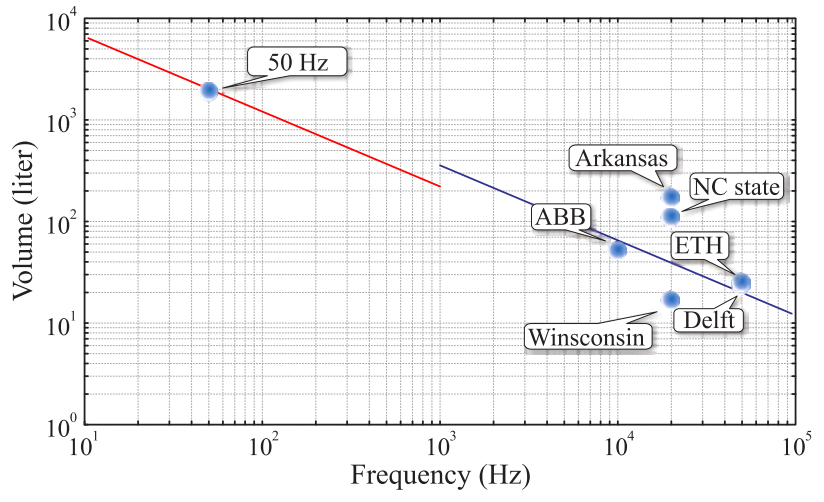
\includegraphics[scale=0.3]{transformer_volume}
    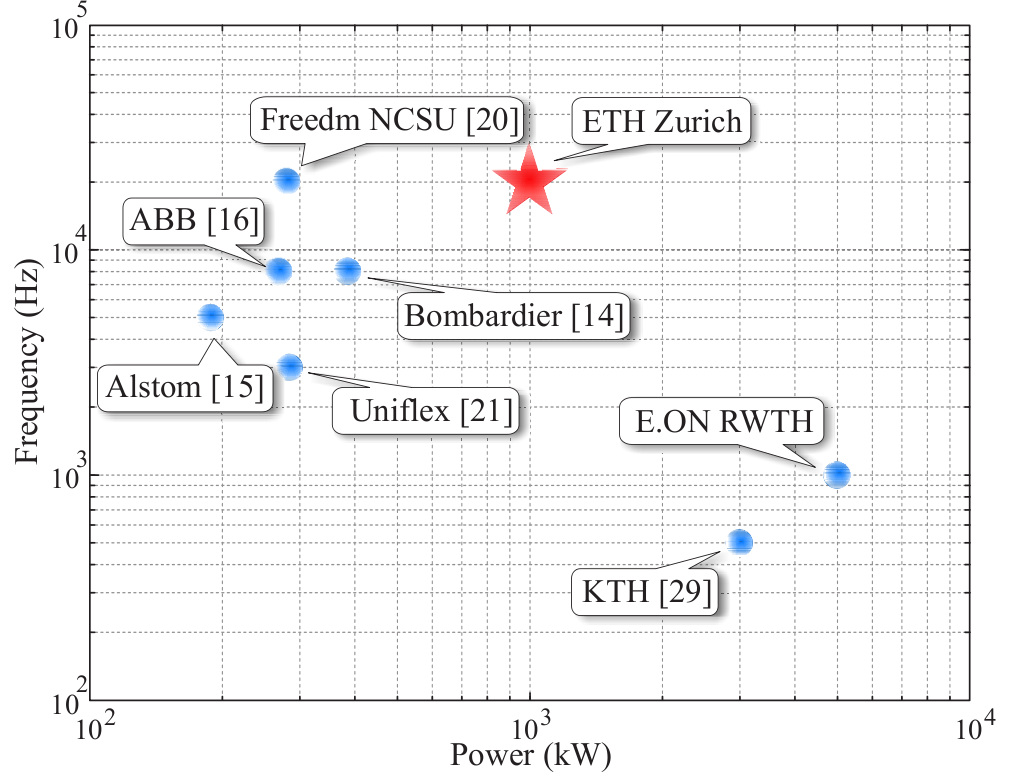
\includegraphics[scale=0.25]{transformer_frequency_commercial_orbitz2010a}
    \caption{Volumes of high frequency transformers(normalized to 1 MW) and rated power and operating frequencies of existing DC-DC converter prototypes \cite{Ortiz2010a,Ortiz2010}.}
  \label{transformer-vols}
\end{figure}


\section{Core Materials}

Although, silicon or nickel-steel laminations are commonly used in conventional line frequency power transformers, the high loss of these components at high frequencies makes other options more viable. Ferrite is one of the first alternatives in the market, but in he recent years materials like amorphous and nanocrystalline become increasingly popular \cite{Agheb2012}.

\subsection*{Amorphous Materials}

Amorphous cores are typically made of Metglas (metalic glass alloy), which is a thin non-crystalline amorphous metal alloy of iron, boron, silicon and phosphorus. The material has a much higher resistivity in electrical steel which results in a low eddy losses. Furthermore, the hysteresis losses of amorphous cores are lower, which reduces the no-load losses compared to one with electrical steel. However, amorphous materials usually have lower saturation flux density compared to conventional iron-silicon electrical steel.

Some manufacturers of amorphous transformer cores can be listed as:

\begin{itemize}
  \item Hitachi Metals (Powerlite)
  \item Vacuumschmelze (Vitrovac)
  \item Metglas
  \item Vijai Electricals
\end{itemize}

Although, amorphous materials are superior to electrical steel laminations, nano-crystalline materials are superior to amorphous materials with their lower cost and higher flux densities \cite{vitroperm_vitrovac}. Nano-crystalline materials will be discussed in the next section. The specifications of amorphous and nano-crystalline materials are compared in Table~\ref{vitropermvitrovac}. The only  application that a amorphous material can be more advantageous is high-frequency single-ended forward converter topologies. For all other topologies, nano-crystalline materials are considered to be more suitable.

\begin{table}[]
\begin{center}
\begin{tabular}{lcc}
 & Amorphous & Nano-crystalline \\ 
 & (Vitrovac) & (VitroPerm) \\
\hline
Saturation Flux Density & 0.8 T & 1.2 T \\
Losses (f= 20 kHz, B=0.2 T) & 2 W/kg & 1.4 W/kg \\
Max. Operating temperature & $110\,^{\circ}\mathrm{C}$ & $120\,^{\circ}\mathrm{C}$ \\
Curie temperature & $365\,^{\circ}\mathrm{C}$ & $600\,^{\circ}\mathrm{C}$ \\
\hline
\end{tabular} 
\end{center}
\caption{Comparison of amorphous (Vitrovac) and nano-crystalline (VitroPerm) materials \cite{vitroperm_vitrovac}.}
\label{vitropermvitrovac}
\end{table}

\subsection*{Nano-crystalline}

Nano-crystalline is a fairly new material that consists of approximately 80\% of iron with the remaining is mixture of silicon, boron, carbon, nickel and other materials. This is a special type of amorphous material, which has superior magnetic characteristics, such as lower core loss and high permeability. Other specifications can be listed as \cite{Magnetics}:

\begin{itemize}
  \item Up to 50 \% permeability than 80\% nickel material (e.g. Supermalloy).
  \item High saturation flux density (1.2-1.5 T).
  \item High operating temperature up to $130\,^{\circ}\mathrm{C}$.
  \item Minimal change of magnetic characteristics with temperature.
  \item 17 \% lighter than Nickel with a density of 7.3 $\mathrm{g/cm^3}$.
  \item Stacking density up to 90 \% can be achieved.
\end{itemize}

Some main manufacturers of nano-crystalline materials can be listed as:

\begin{itemize}
  \item MK Magnetics
  \item Vacuumschmelze
  \item Hill-Tech
\end{itemize}

In this section, different types of nano-crystalline materials will be compared. 
Vacuumschmelze manufactures various soft magnetic nano-crystalline materials under the brand of VitroPerm.


\subsubsection*{VitroPerm}

Nanocrystalline VitroPerm alloys are based on Fe with Si and B with Nb and Cu additives \cite{vitroterm_manual}. VitroPerm nano-crystalline alloys are optimized to combine highest permeability and lowest coercive field strength. The combination of very thin tapes and the relatively high electrical resistance (1.1-1.2~$\mu \Omega m$) to ensure minimal eddy current losses and an outstanding frequency vs. permeability behaviour. Along with saturation flux density of 1.2 T and wide operational temperature range, these features combine to make VitroPerm  superior in many aspects to commonly used ferrite and amorphous materials. Magnetization curves and B-H characteristics of VitroPerm materials are presented in Fig.~\ref{vitroterm_BH}.

\begin{figure}[]
  \centering
    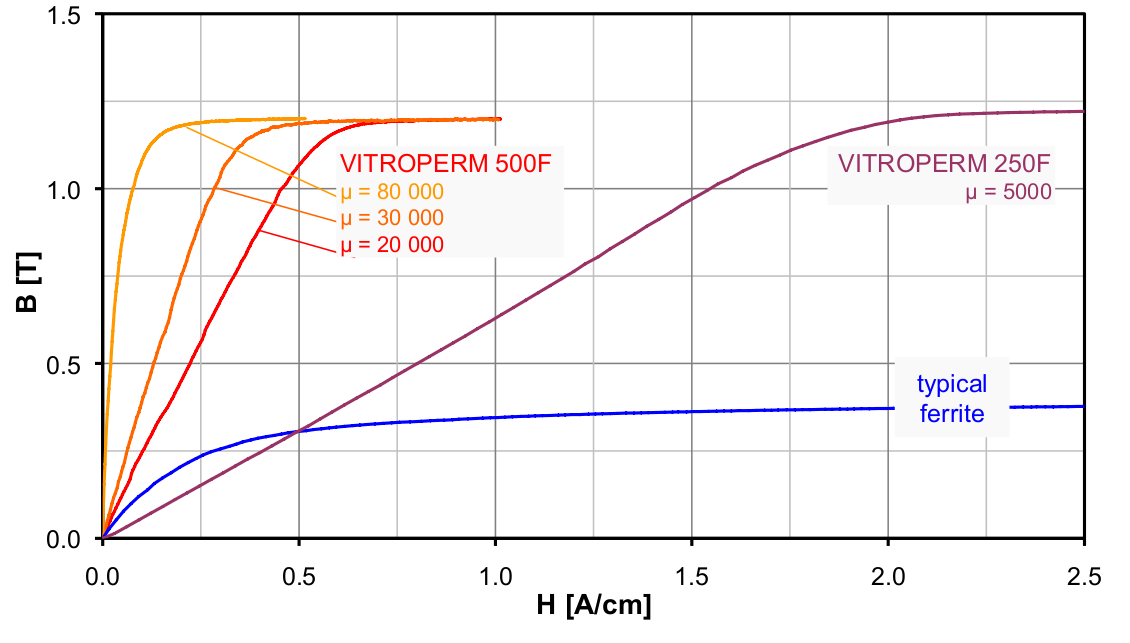
\includegraphics[scale=0.3]{vitroperm_magnetization}
    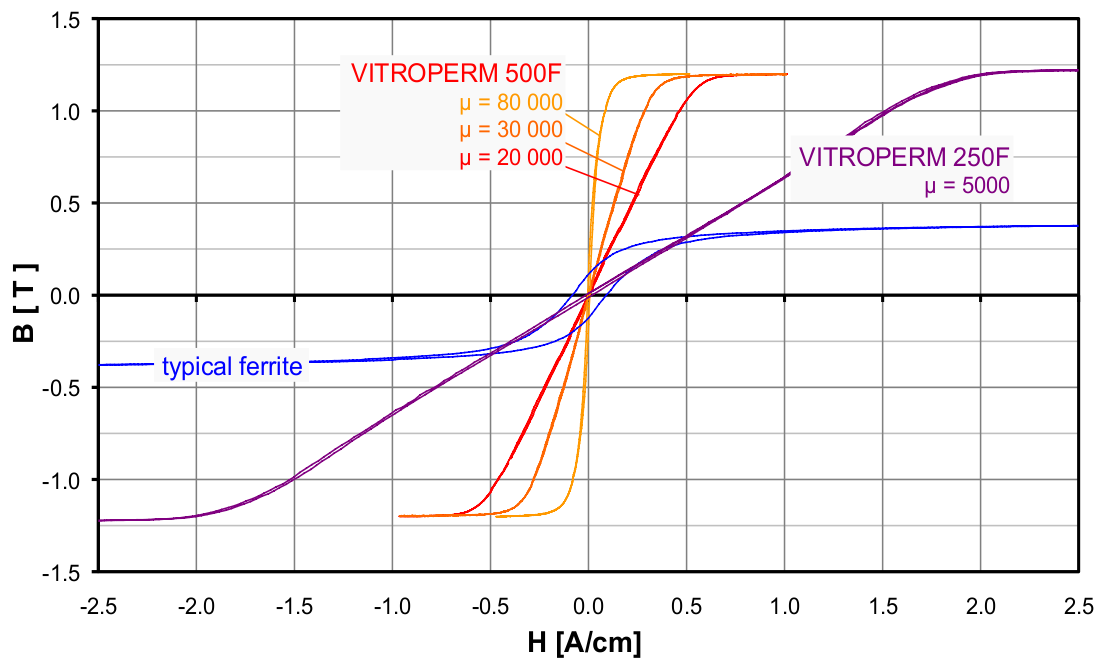
\includegraphics[scale=0.3]{vitroterm_hysteresis}
    \caption{Magnetisation curve and B-H characteristics of VitroPerm \cite{vitroterm_manual}.}
  \label{vitroterm_BH}
\end{figure}

VitroPerm has a wide range material options with different permeability scale as as shown in Fig.~\ref{vitroterm_permeability}. 
The permeability of VitroPerm 500F is significantly higher than ferrite as shown in Fig.~\ref{vitroperm500_250_permeability}.

\begin{figure}[]
  \centering
    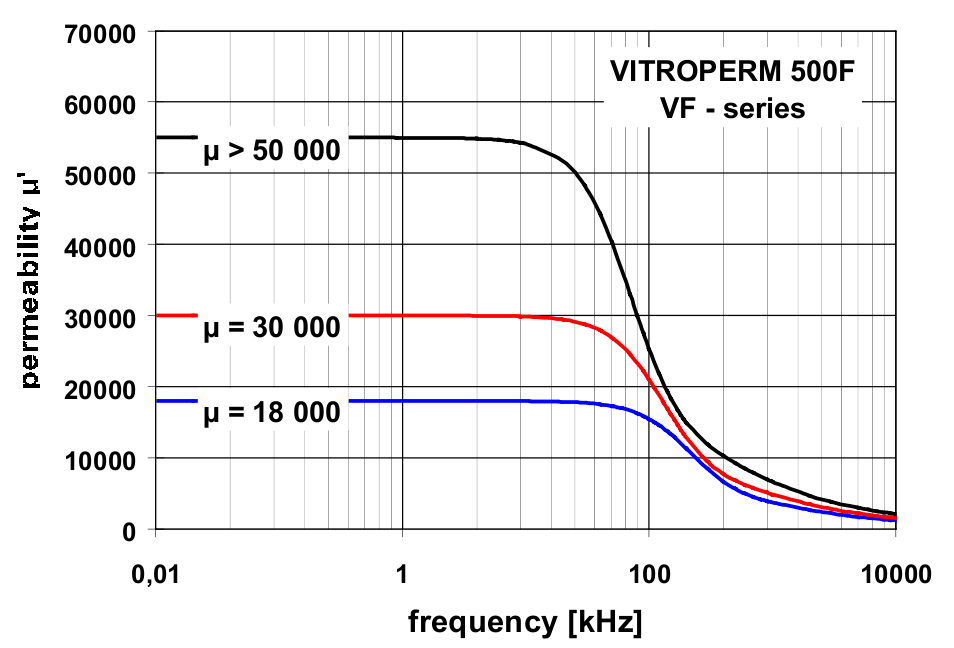
\includegraphics[scale=0.3]{vitroterm_permeability}
  \caption{Permeability change of different VitroPerm materials with frequency \cite{vitroperm_toroidal}.}
  \label{vitroterm_permeability}
\end{figure}

\begin{figure}[]
  \centering
    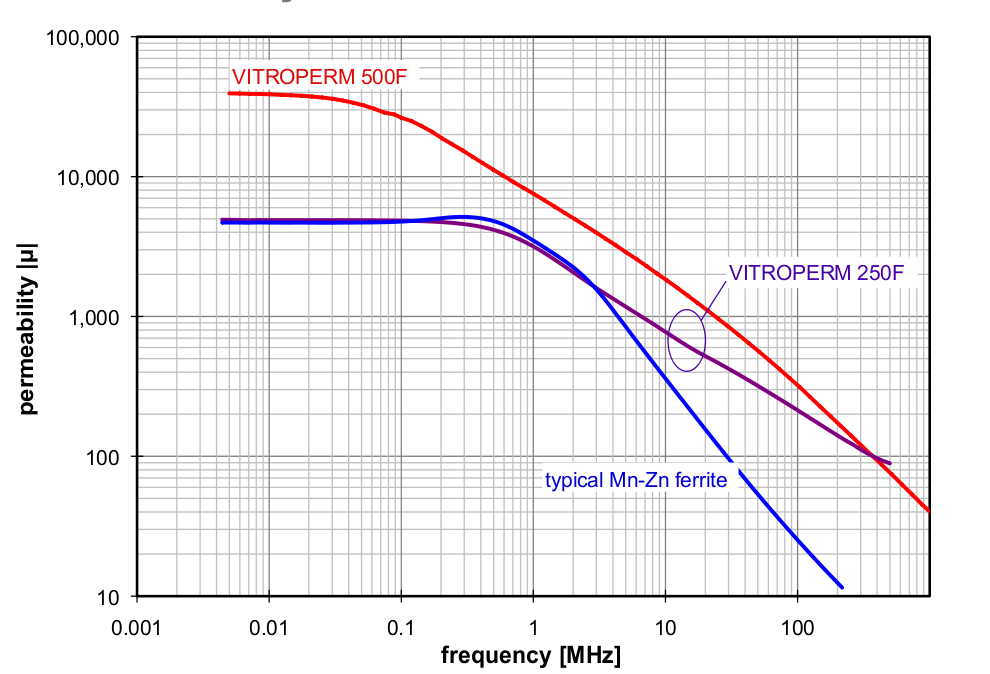
\includegraphics[scale=0.3]{vitroperm500_250_permeability}
  \caption{Permeability change of VitroPerm 250F($\mu = 5000$), VitroPerm 500F($\mu = 40000$) and ferrite($\mu = 5000$) with frequency. \cite{vitroterm_manual}.}
  \label{vitroperm500_250_permeability}
\end{figure}

VitroPerm has also a high operating temperature compared to ferrite. The Curie temperature of VitroPerm alloys are $600\,^{\circ}\mathrm{C}$. Furthermore, the saturation flux density only reduces by 10\% at $120\,^{\circ}\mathrm{C}$, which allows the core can be overloaded for short-amount of periods up to $180-200 \,^{\circ}\mathrm{C}$. The variation of permeability with temperature for VitroPerm is presented in Fig.~\ref{temp_vs_saturation}.

\begin{figure}[]
  \centering
    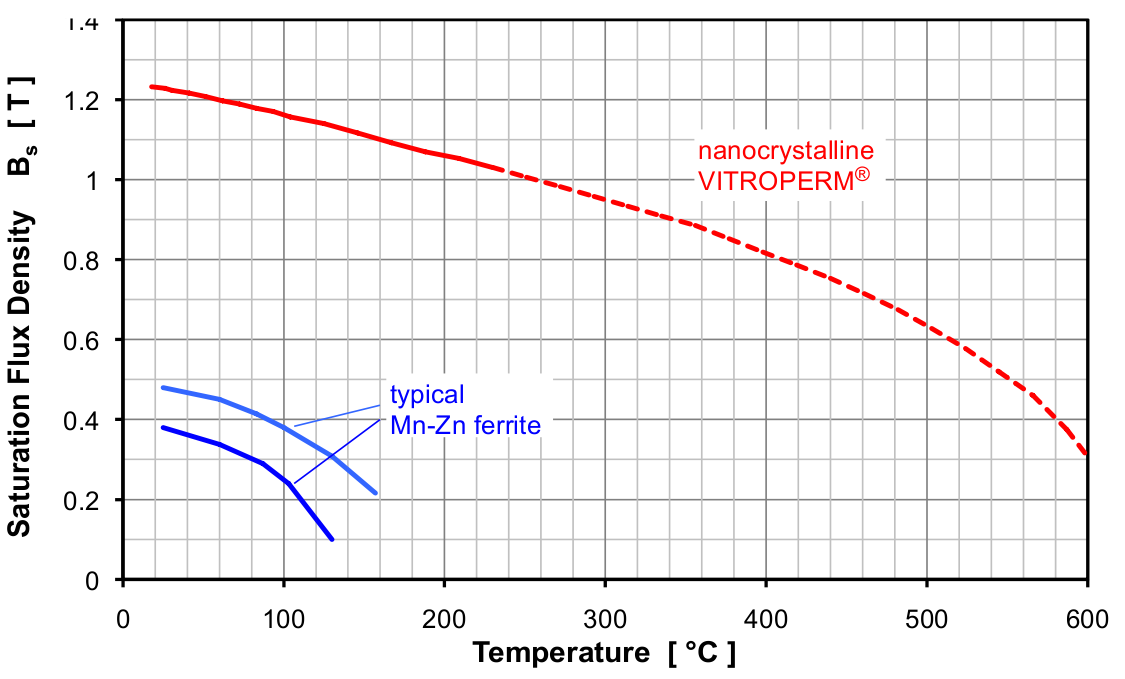
\includegraphics[scale=0.3]{temp_vs_saturation}
  \caption{Saturation flux density variation of VitroPerm with temperature.}
  \label{temp_vs_saturation}
\end{figure}

\subsection*{Silicon-Steel}

Silicon-steel is a popular choice in line frequency power transformers for its low cost and high-saturation magnetic induction. However, core losses of silicon-steel is high compared to other materials, which makes them unsuitable for medium frequency transformers. The core losses of material will be compared in the next section.

\subsection*{Ferrites}

Ferrites have a low-loss density in very high-frequencies, which makes them a suitable material for high-frequency applications such as RF-filters and chokes. However, they have saturation flux density around 0.5 T, which increases the core volume and mass in high power applications. 

\subsection*{Core Material Comparison}

Different core materials and manufacturers are presented in Table~\ref{core-loss-table}. In Fig.~\ref{material_table}, prototypes with common core materials are presented. It can be seen from the table that nano-crystalline and amorphous materials are the most suggested materials for medium frequency transformers that work between 1 kHz and 25 kHz.

\begin{table}[]
\begin{center}
\begin{tabular}{llccl}
 Material & Brand & Saturation Flux & Core Loss & Manufacturer \\ 
 \hline
& Microlite & 1.56 T & 1.5 kW/kg & Metglas\\
Amorphous & Powerlite & 1.56 T & 0.6 kW/kg & Metglas\\
& Namglass & 1.59 T & 0.34 kW/kg & Magmet\\
& Vitrovac & 0.82 T & 0.19 kW/kg & VAC\\
\hline
& Finemet & 1.23 T & 0.14 kW/kg & Hitachi\\
Nano-crystalline& VitroPerm & 1.2 T & 0.07 kW/kg & VAC\\
& Nanoperm & 1.2 T & 0.04 kW/kg & Magnetec\\
& Namglass 4 & 1.23 T & 0.04 kW/kg & Magmet\\
\hline
Silicon Steel & Arnon 7 & 1.53 T & 1.6 kW/kg & Arnold\\
& Arnon 5 & 1.48 T & 1.06 kW/kg & Arnold\\
\hline
\end{tabular} 
\end{center}
\caption{Core materials and manufacturers for high-frequency transformers (specific losses at B = 1 T, f = 20 kHz) \cite{Ortiz2010}.}
\label{core-loss-table}
\end{table}


\begin{figure}[]
  \centering
    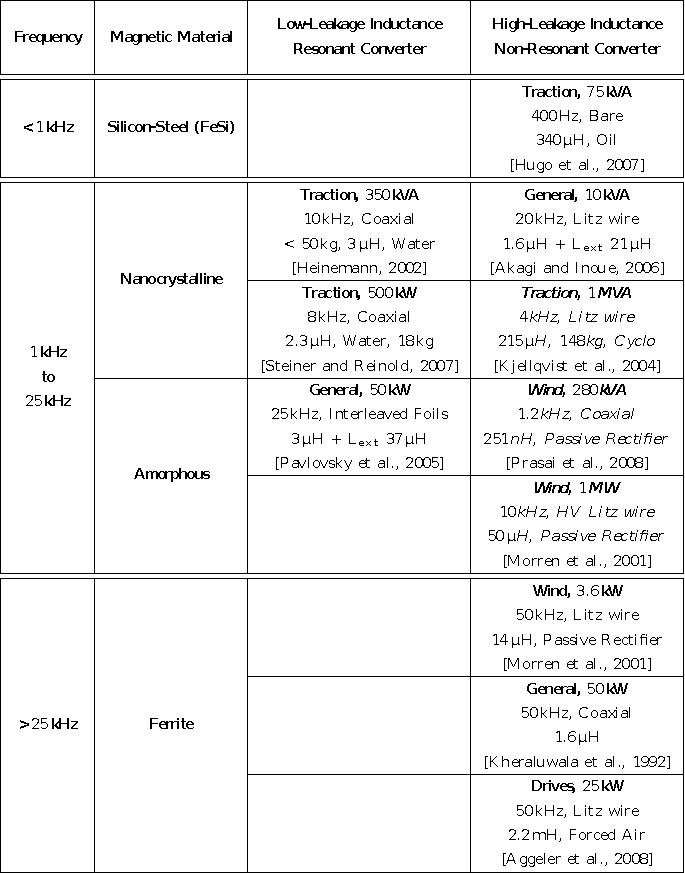
\includegraphics[]{material_table_villar_2010}
  \caption{Common materials used in medium frequency transformers and previous prototypes (Heinemann, 2002:\cite{Heinemann2002}, Steiner,2007:\cite{Steiner2007}, Pavlovsky,2005:\cite{Pavlovsky2005}, Morren,2002:\cite{Morren2002}, Prasai,2007:\cite{Prasai2007}) \cite{Villar2010}.}
  \label{material_table}
\end{figure}

The hysteresis losses and the core loss of different materials are compared in Fig.~\ref{core-loss}. Core losses are presented in Fig.~\ref{core-loss-log}. It can be seen that between 1 kHz and 10 kHz, the core loss of 0.3 mm silicon-steel laminations are 25 times higher than nano-crystalline material. 
A 50 kV, high frequency (20 kHz), 150 kW transformer that uses nano-crystalline material is presented in \cite{Filchev2009}, in which the core losses are estimated as 60W/kg at an operating flux density of 1 T.

\begin{figure}[]
  \centering
    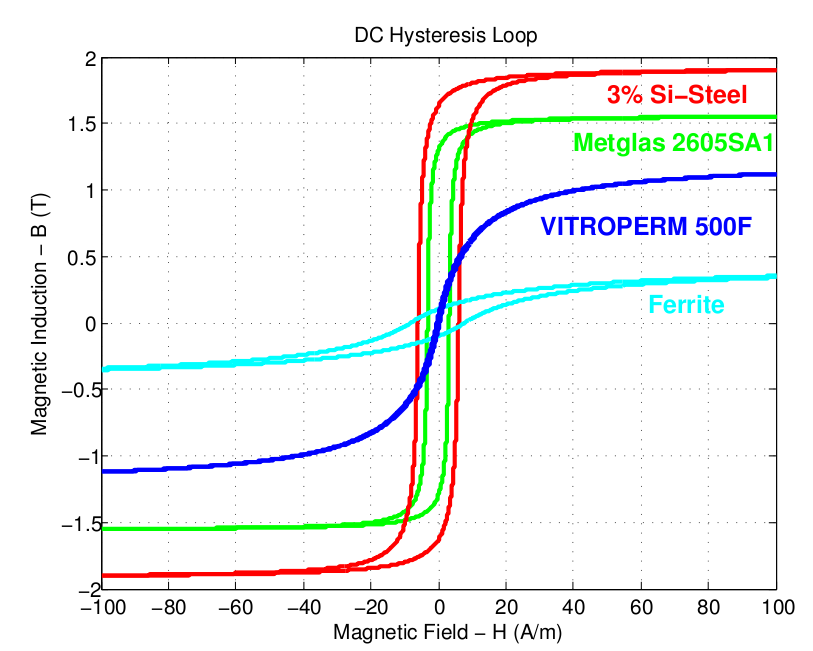
\includegraphics[scale=0.3]{hysteresis-losses}
    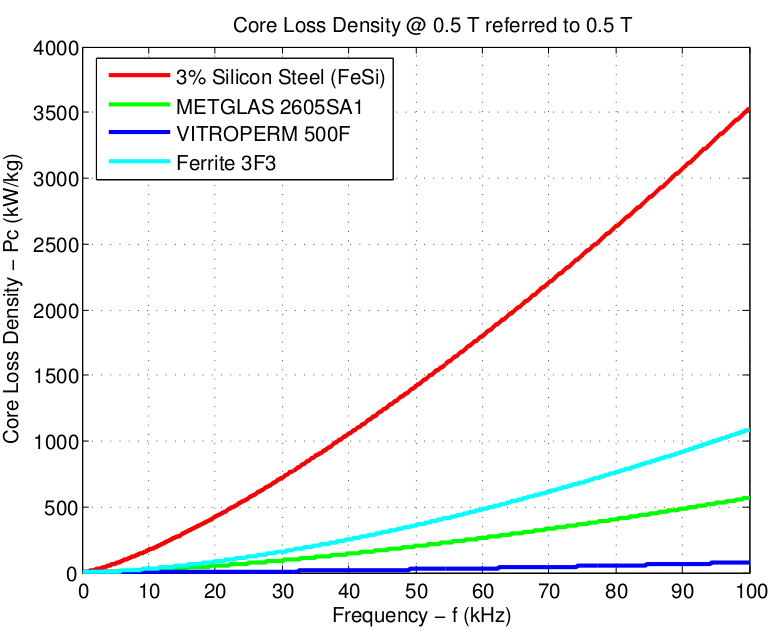
\includegraphics[scale=0.3]{core-loss}
  \caption{Loss comparison of silicon-steel, amorphous, nano-crystalline and ferrite materials \cite{Villar2010}. a) Hysteresis loss, b) Core loss.}
  \label{core-loss}
\end{figure}

\begin{figure}[]
  \centering
    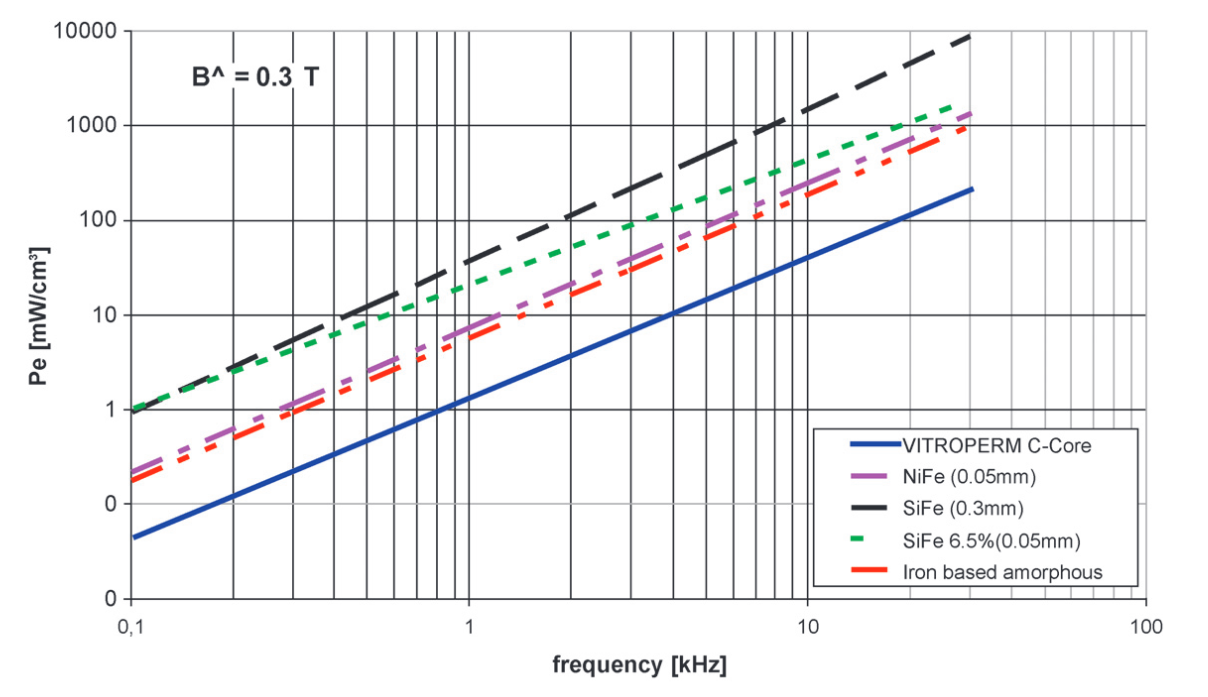
\includegraphics[scale=0.3]{vitroperm_core_losses_vs_freq}
  \caption{Core loss comparison of nano-crystalline (VitroPerm) with electrical steel and amorphous material \cite{vitroterm_manual}.}
  \label{core-loss-log}
\end{figure}

\section{Losses in a Transformer}

There are many analytical models to calculate the losses of medium frequency transformers. These methods, for different transformers types are reviewed in \cite{Agheb2012} and in \cite{Villar2010}.

\subsection{AC Winding Losses}

The high frequency excitation in a medium frequency transformer has two main effects in the transformer windings:
\begin{itemize}
  \item Skin Effect: In AC excitation the current itself generates an opposing magnetic field and current, which reduce the net current density inside the conductor. The total current will stay same, but the distribution will be higher across the circumference of the conductor.
  \item Proximity Effect is the interaction between two adjacent conductors that alters the current distribution in the conductor. Same principles(e.g. proximity, frequency) apply in the proximity affect.
\end{itemize}

Losses due to skin effect decrease by increasing the foil thickness whereas proximity effect losses increase with increasing foil thickness \cite{Ortiz2010}.

\subsubsection{Skin Effect}

Skin effect is an important factor in AC resistance and eddy current losses in a transformer. Skin effect is effected by the skin depth, which can be expressed as:

\begin{equation}
  \sigma = \sqrt{\frac{2\rho}{\mu \omega}}
\end{equation}

where $\rho$ is the resistivity of the conductor, $\mu$ is permeability, and $\omega$ is the frequency in rad/s. Skin depth of copper for different operating frequencies are presented in Table~\ref{skin-depth}. For reasonable AC resistance characteristics, the rule of thumb is to choose the conductor diameter smaller than 1.6 times of the skin depth. Thus, for a 1-2 kHz transformer application, the conductor should not be thicker than 2-3 mm. 

\begin{table}[]
\begin{center}
\begin{tabular}{cc}
Frequency & Skin Depth \\
\hline
50 Hz & 9.2 mm \\
1 kHz & 2.06 mm \\
2 kHz & 1.49 mm \\
5 kHz & 0.94 mm \\
10 kHz & 0.65 mm \\
50 kHz & 0.29 mm \\
\hline
\end{tabular} 
\end{center}
\caption{Skin depth in a copper conductor.}
\label{skin-depth}
\end{table}

In a step-up transformer the cross-section area of the primary conductor will be larger. However, the limit due to skin-depth limits the thickness of the conductor. Therefore, the most feasible way is to use foil conductors in the primary windings. 
Dowell calculated eddy losses in foil type transformer windings in \cite{Dowell1966}. A detailed explanation of these one dimensional Maxwell equations can be found in \cite{Villar2010} and a summary will be presented in this section.

The DC resistance of a foil winding can be expressed as:

\begin{equation}
  R_{dc} = \rho \frac{L_{mean}}{t_w h_w} N_{turns}
\end{equation}

where $L_{mean}$ is the mean turn length of the coil, $t_w$ is the thickness, $h_w$ is the height, $\rho$ is the resistivity of copper.

The AC resistance is more complicated to calculate and depends on the ratio of the wire thickness to skin depth ($\delta$) and can be expressed as:

\begin{equation}
  R_{ac}=\rho \frac{L_{mean}}{h_w \delta} N_{turns} \left[\varsigma_1 + \frac{2}{3} (N_{turns}^2-1)\varsigma_2\right]
  \label{R_ac_foil}
\end{equation}

where:

\begin{equation}
  \varsigma_1 = \dfrac{sinh(2\Delta)+sin(2\Delta)}{cosh(2\Delta)-cos(2\Delta)} \quad
  \varsigma_2 = \dfrac{sinh(\Delta)-sin(\Delta)}{cosh(\Delta)+cos(\Delta)} \quad  
  \Delta = \dfrac{t_w}{\delta}
\end{equation}

as can be seen from the equation above,  the important factor is the penetration factor (i.e the ratio of conductor thickness to skin depth, $\Delta$). The ratio of AC resistance to DC resistance is called Dowell's resistance factor ($F_r$). The resistance factor as a function of penetration ratio for a 2 mm thick foil wire is presented in Fig.~\ref{resistance_factor}. For example, at 1 kHz the skin depth is 2.1 mm (the penetration ratio is approximately 1), the resistance factor is 2.7 for a layer number of 4. Thus the resistive losses will be 2.7 times more compared to DC conduction.

\begin{figure}[]
  \centering
    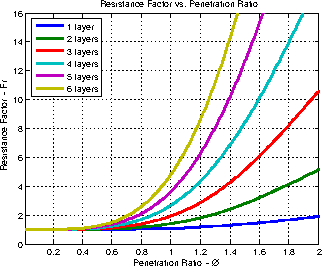
\includegraphics[scale=1.25]{resistance_factor}
  \caption{Resistance factor for a function of penetration ratio (for 2 mm thick foil conductor) \cite{Villar2010}.}
  \label{resistance_factor}
\end{figure}

\subsubsection{Secondary-Winding}

There are different analytical models to estimate the AC resistances of round conductors (e.g. high voltage cables that can be used in the secondary winding), such as presented in \cite{Sullivan2003,Ferreira1994}. Although, the method presented by Dowell in \cite{Dowell1966} is assumed as the most established method. In this method Dowell introduced a porosity factor to convert the round conductors to square conductors and then convert to foil type conductors.

Equivalent thickness of a round conductor can be defined as \cite{Dowell1966}:

\begin{equation}
 d_w =  \sqrt{\frac{\pi}{4}} d 
\end{equation}

where $d$ is the diameter of the round conductor and $d_w$ is the thickness of the equivalent square conductor. Then, similar technique can be applied to convert square conductor to foil type conductor using a second porosity factor as shown in \cite{Villar2010}. Therefore, the AC resistance of the round conductor can be expressed similarly to equation (\ref{R_ac_foil})) as given in \cite{Villar2010}.


\section{Core Losses}

The core losses mainly depend on the material type, flux density and operating frequency. Although, there are many methods to estimate the core losses as reviewed in \cite{Shen2006}, the most common method is to use a power equation, which is known as the Steinmetz equation:

\begin{equation}
 P_{core} = K f^a B^b
\end{equation}

where $f$ is the operating frequency, $B$ is peak magnetic flux density, $K$, $a$ and $b$ are factors determined by the material characteristic obtained from the manufacturer's data.

Steinmetz equation is usually well established method for line transformers, in which sinusoidal excitation is used. However, in the medium-high frequency transformers, the transformer is excited using power electronics (usually a square waveform, or stepped waveform), and transformer voltage and current include many harmonics.


\subsection{Core Losses in Non-Sinusoidal Excitation}

Various methods are developed to model the core losses under non-sinusoidal excitation \cite{Venkatachalam2002,Reinert2001}. Some of the methods reviewed in \cite{Villar2010} can be listed as:

\begin{itemize}
\item	Modified Steinmetz Equation
\item	Improved Generalized Steinmetz Equation
\item	Equivalent Elliptical Loop
\item	Waveform Coefficient Steinmetz Equation
\end{itemize}

In \cite{Venkatachalam2002}, a model has been developed to predict the non-sinusoidal excitation losses using just the standard Steinmetz parameters. The model calculates the total loss by adding the losses in major and minor loops in the voltage waveform.

Although these methods can provide more accurate results compared to Fourier transform method, they all require extra measurement steps to determine the material characteristics at different operating frequencies and waveforms. Therefore, it is impractical to use these models without experimental study at first. Therefore, using standard Steinmetz equation with harmonics contents is an ideal choice for analytical core loss estimation.

For non-sinusoidal waveforms, the easiest way to calculate the core losses is to use Fourier transform to get the frequency components and then to estimate individual core losses for each component. 

The transformer developed by Narec will be excited using a square waveform in the low voltage side, and a multi-level inverter will be used in the high voltage side.

The core losses resulting from the low-voltage square wave excitation can be calculated by expressing the square wave as a Fourier series:

\begin{equation}
 f(x) = \frac{4}{\pi} \sum_{n=1,3,5...}^{+\infty} \frac{1}{n} sin ( n \omega x )
\end{equation}

where $\omega$ is the frequency of the square waveform in radians/s, $n$ is the harmonic order. The magnitudes of the Fourier series components of the square wave relative to the magnitude of the square wave is presented in Table~\ref{square_harmonics}.

\begin{table}[]
\begin{center}
\begin{tabular}{ll}
Harmonic Order & Magnitude\\
\hline
1 & 1.273\\
3 & 0.424 \\
5 & 0.254 \\
7 & 0.182 \\
9 & 0.141 \\
11 & 0.116 \\
13 & 0.098 \\
\hline
\end{tabular} 
\end{center}
\caption{Fourier series magnitudes relative to the magnitude of the square wave.}
\label{square_harmonics}
\end{table}


\section{Modeling of the Transformer}

A Matlab model is developed to estimate the transformer models and calculate copper and core losses. The design methodology used in the Matlab code is depicted in Fig.~\ref{design_method}.

\begin{figure}[]
  \centering
    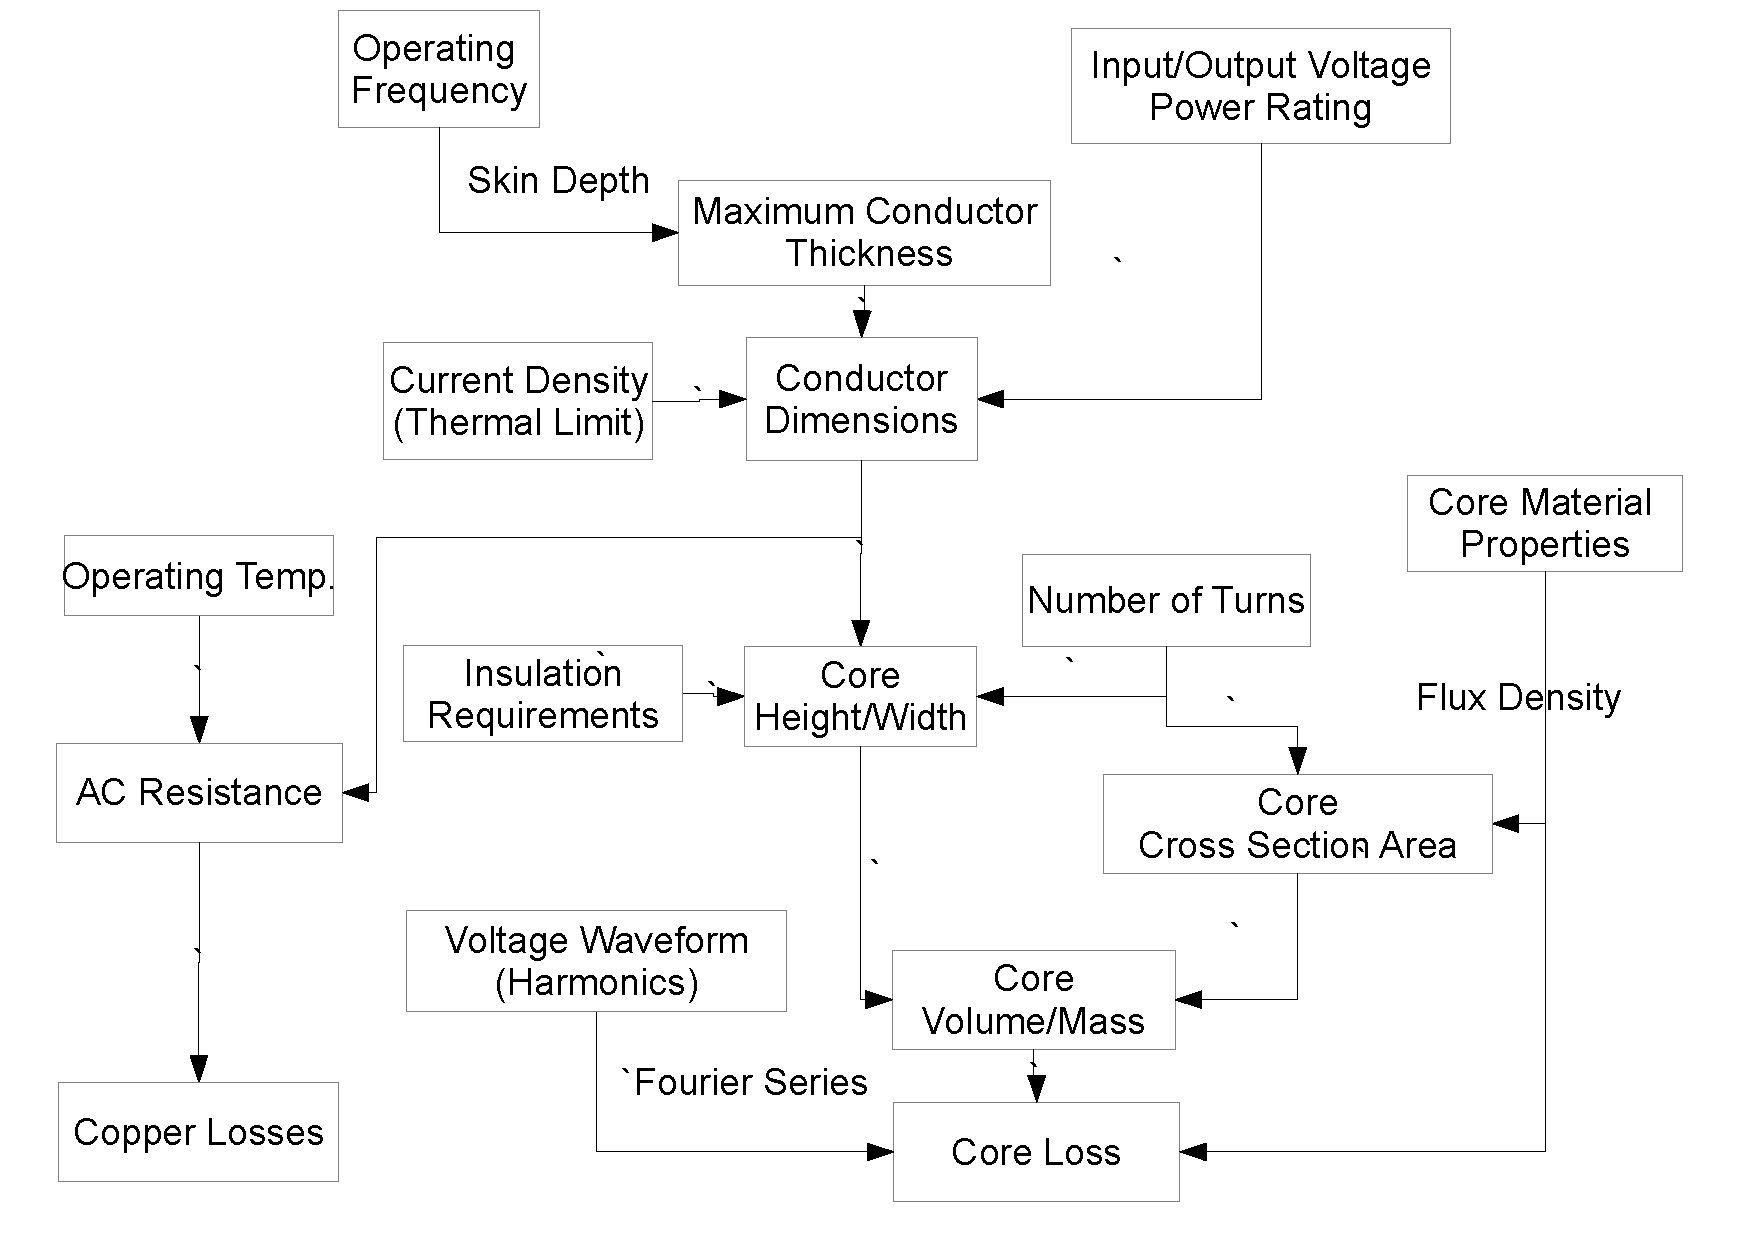
\includegraphics[scale=0.4]{design_method}
  \caption{Design methodology to estimate transformer parameters and losses.}
  \label{design_method}
\end{figure}

\subsection{Estimation of Winding Parameters}

It is assumed from the WP 2 report that, foil type conductors are the most suitable option for the low voltage side. On the high voltage side, circular stranded cables are more suitable with their mechanical strength and increased dielectric insulation. It is stated in \cite{Morren2002} that, using standard high-voltage cables has advantages such as: elimination of oil insulation, and better distribution of electric field in round conductors. 

The thickness of the coil is chosen according to the skin depth at the operating frequency. The conductor thickness is selected to be less than 1.5 times skin depth, however, actual foil conductor thickness is limited to standard wire gauges (e.g. 1 mm, 1.6 mm, 2 mm, 2.25 mm...). The frequency of the transformer versus the most suitable foil coil thickness is plotted in Fig.~\ref{primary_thickness}. For example, for operating frequencies between 2 kHz and 3 kHz, the most suitable conductor thickness is 2 mm.


\begin{figure}[]
  \centering
    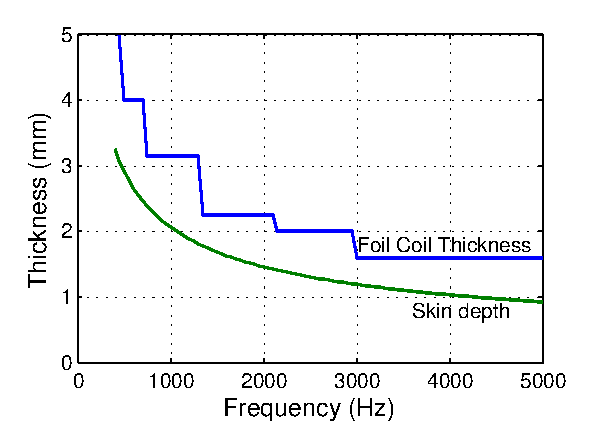
\includegraphics[]{primary_thickness}
  \caption{Skin depth and primary foil winding size variation (Standard foil conductor sizes are used).}
  \label{primary_thickness}
\end{figure}


Then, using rated current and the rated current density, the required conductor area can be calculated. The conductor height can be found by dividing the conductor area to conductor thickness. For example, assuming a current density of $4 A/mm^2$, the foil conductor height can be calculated as a function of the operating frequency as shown in Fig.~\ref{primary_height}.

Similar method can be used for the secondary HV winding, where a standard circular HV cable can be used. The standard diameter of these cables are 2.5 mm, 4 mm, 6 mm, 10 mm, 16 mm. More information about HV cables can be found in \cite{HVcable}.


\begin{figure}[]
  \centering
    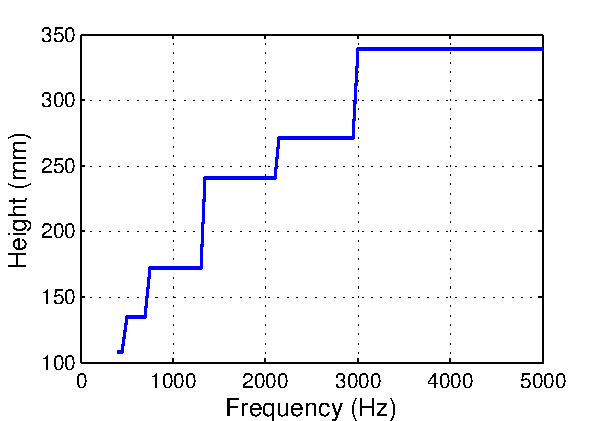
\includegraphics[]{primary_height}
  \caption{Height of the foil conductor as a function of the operating frequency.}
  \label{primary_height}
\end{figure}

Insulation parameters should be known to determine the dimensions of the primary and secondary windings. Dry insulation is considered to be the most suitable insulation type due to increased reliability and ease of manufacturing. However, oil flooded windings can be preferred to improve thermal performance.  In Table~\ref{dielectric}, dielectric strengths of some common dry-type insulation materials are presented and typical insulation thickness values are presented in \cite{Ortiz2010}. Although, type of the insulation material is not specified in this report, but it is stated in WP2 report that the most suitable insulation type is potted epoxy. Following insulation thickness values are chosen to calculate AC copper losses. In order to get more accurate results, these values should be modified in the model once the detailed design of the transformer is completed.

\begin{table}[]
\begin{center}
\begin{tabular}{lcc}
Insulation Type & Material & Dielectric Strength\\
\hline
Potted & Epoxy & 16 kV/mm\\
Potted & Micares & 8-24 kV/mm \\
HV Cable & Silicone & 4-28 kV/mm\\
HV Cable & PVC & 10-10 kV/mm\\
HV Cable & HDPE & 19 kV/mm \\
\hline
\end{tabular} 
\end{center}
\caption{Dry-type insulation dielectric strengths \cite{Ortiz2010}.}
\label{dielectric}
\end{table}

\begin{itemize}
\item Insulation thickness between primary (low voltage) conductors: 1 mm
\item Insulation thickness from primary winding to core: 10 mm
\item Outer insulation thickness around primary winding: 10 mm
\item Insulation thickness between secondary (high voltage) conductors: 5 mm
\item Insulation thickness from secondary winding to core: 20 mm
\item Outer insulation around secondary winding: 20 mm
\item Insulation thickness between primary and secondary windings: 50 mm
\end{itemize}

\subsection{Estimation of Core Dimensions}

The most important parameter of the core is the cross-section area, which depends on the operating frequency, flux density in the core and the number of turns. Assuming a square cross-section area, the thickness of the core as  a function of the primary number of turns is estimated as in Fig.~\ref{core_dimensions}, and similarly graphs for the secondary number of turns are presented in Fig.~\ref{secondary_core_dimensions}. The operating flux density of the core is assumed as 1.1 T, the primary voltage magnitude is assumed as 3 kV, and the secondary voltage magnitude is assumed as 300 kV.

Although, it is not presented in this report, the main dimensions and the mass of the core is calculated in the Matlab models and these figures can be used to estimate the overall weight and cost of the transformer.

\begin{figure}[]
  \centering
    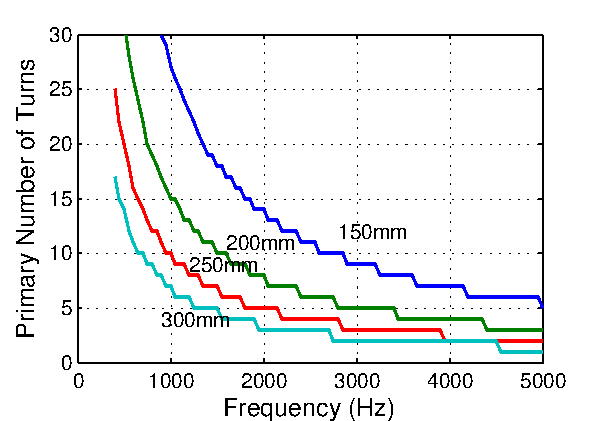
\includegraphics[]{primary_Nturns_core}
    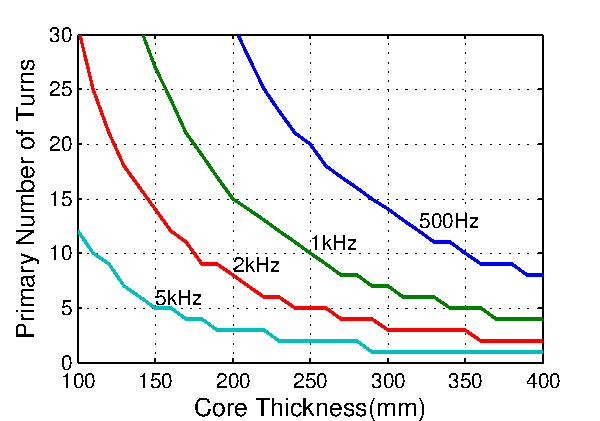
\includegraphics[]{primary_Nturns_freq}
  \caption{Core-thickness (assuming square cross-section area) as a function of the primary number of turns and operating frequency (B=1.1 T, Vin=3 kV, Vout=300 kV).}
  \label{core_dimensions}
\end{figure}


\begin{figure}[]
  \centering
    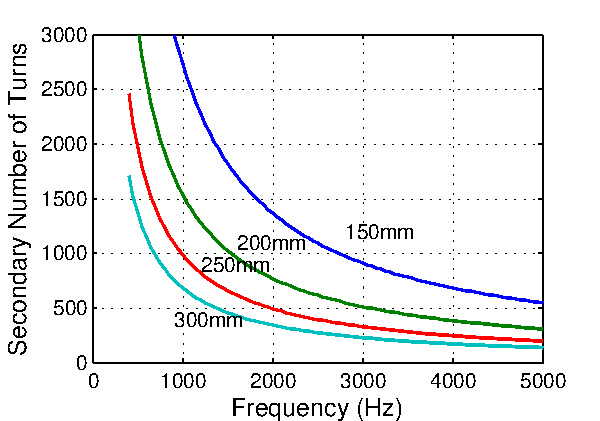
\includegraphics[]{secondary_Nturns_core}
    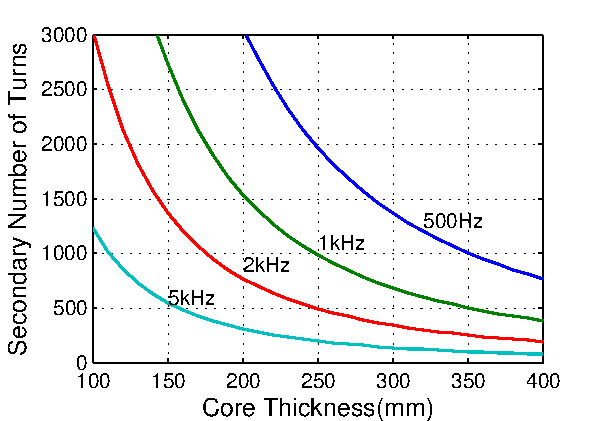
\includegraphics[]{secondary_Nturns_freq}
   \caption{Core-thickness (assuming square cross-section area) as a function of the secondary number of turns and operating frequency (B=1.1 T, Vin=3 kV, Vout=300 kV).}
  \label{secondary_core_dimensions}
\end{figure}


\section{Conclusion}

In this report, a review of core materials and loss calculation methods for medium frequency transformers are presented. Following conclusions can be drawn from the report:

\textbf{Core Material}: Although electrical steel laminations are commonly used in line frequency transformers, they are not suitable in medium frequency transformers with their increased losses. Ferrites have very low losses, but they also have a very low operating flux density, which makes them unsuitable for high power applications. Nano-crystalline material is considered to be most suitable material with its high flux density and very low losses at high frequencies. Vacuumschmelze's Vitroperm500F is a popular material, that can be used. Amorphous materials can be used to reduce the core mass, as their operating flux densities are 25\% higher than nano-crystalline materials, but they have higher losses.

\textbf{Core Type}: Various transformer core topologies are compared in \cite{Agheb2012}. It is considered that core type transformer is the simplest and easiest to manufacture, and hence the most suitable option as the initial prototype.

\textbf{Winding Type}: In the primary field windings, the most suitable winding type is foil-type conductors, as low thickness is required for minimum eddy current loss, but a large conductor area is required to conduct high input current. It is possible to use two parallel primary windings to double the conducting area. Standard HV cables are proposed to be used in the secondary winding in order to simplify the manufacturing and insulation.Multi-stranded insulated conductors can be used to minimize the eddy current losses as a replacement to Litz wires.

Matlab models are developed to estimate basic dimensions of the transformer core and winding. These parameters can be used as an input to finite element models or for a more detailed analytical models. In order to calculate the core losses accurately, the loss mapping of the material with magnetic flux and operating frequency should be known. This can be obtained from the manufacturer directly for some common materials, but a better option is to setup a small experimental rig to obtain these values.

\clearpage

\section{Sample Design}

In this section, four transformer designs will be presented with different primary number of turns. The initial designs are developed the Matlab model described in the previous section.

The main dimensions in the analytical design are presented in Fig.~\ref{transformer_dimensions}.

\begin{figure}[]
  \centering
    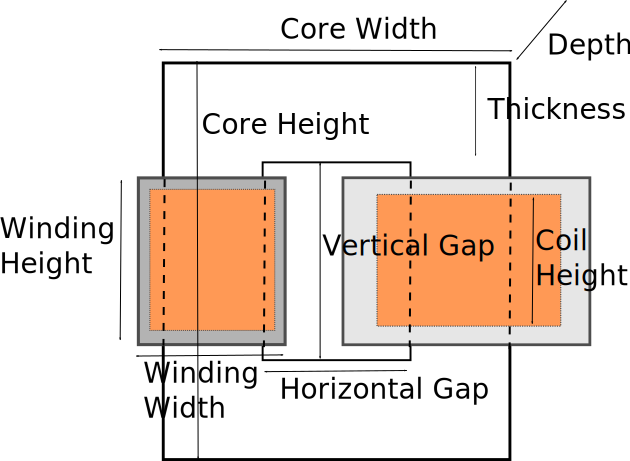
\includegraphics[width=0.5\textwidth]{transformer_dimensions}
   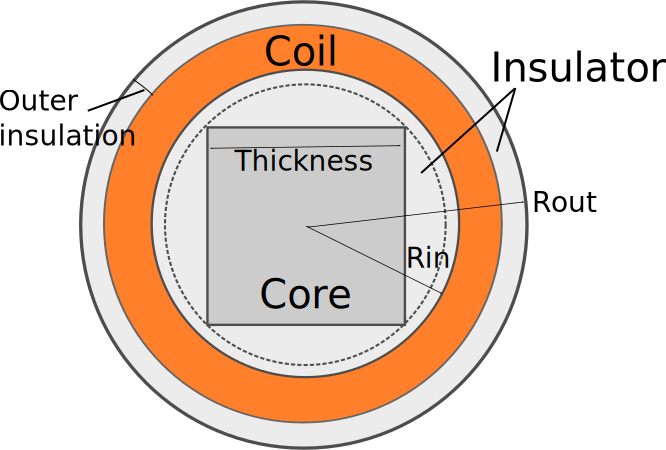
\includegraphics[width=0.45\textwidth]{transformer_dimensions_cross_section}
  \caption{Main dimensions of the transformer. a) Side-view, b) Cross section of the core and winding.}
  \label{transformer_dimensions}
\end{figure}

Following assumptions are made in the design process:

\begin{itemize}
\item Operating Frequency: 1 kHz
\item Core Material: Vitroperm 500F
\item Operating Flux Density: 1.1 T (90\% of the saturation flux density)
\item Operating  Temp: 110 C (for resistance calculations)
\item Current Density: 4 A/mm$^2$ (in the conductor).
\item Permeability: $\mu = 30000$
\item Core Type: C-core with square cross-section.
\item LV Coil Type: Foil type conductor. The thickness is calculated considering eddy current loss as described in the previous section.
\item HV Coil Type: Round insulated HV cable.
\item Inner Insulation Thickness(Insulation between winding and the core): 6 mm for the low-voltage side, 20 mm for the high-voltage side.
\item Outer Insulation Thickness: 10 mm for the low-voltage side, 20 mm for the high-voltage side.
\item Insulation Thickness Between Conductors: 1 mm for the primary coil, 5 mm for the secondary.
\item Gap Between LV and HV Winding: 50 mm
\end{itemize}

Four Designs are presented in this report with varying primary(low-voltage) number of turns:

\begin{itemize}
\item Design A: $Nturns_{LV}=5$
\item Design B: $Nturns_{LV}=8$
\item Design C: $Nturns_{LV}=12$
\item Design D: $Nturns_{LV}=15$
\end{itemize}

The specifications of these designs are presented through Table~\ref{design_A} to Table~\ref{design_D}. Core mass, LV and HV conductor length variation are presented in Table~\ref{conductor_length}. From the table, following can be concluded:
\begin{itemize}
\item Core mass reduces as the number of turns increases.
\item The length of both windings increase with number of turns. However, increase in the LV winding length is less compared to HV winding length. For example, when primary number of turns is increased from  5 to 15, the length of the LV winding just doubles, however, the length of HV winding quadruples, which makes the losses in the HV side more dominant. This is due to thick insulation around the HV cable and high number of turns.
\item Assuming the core loss is proportional to core mass and the copper loss is proportional to conductor length, the core loss reduces with increasing number of turns, whereas the copper loss increases with increasing number of turns.
\end{itemize}

The optimum number of turns is selected as 8 for the FEA simulations. FEA simulations are performed with Opera 3D software and the model building scripts can be found in the project folder.

\begin{table}[]
\begin{center}
\begin{tabular}{lcccc}
& $Nturns_{LV}$ & LV Winding & HV Winding & Core Mass \\
\hline
Design A & 5 & 8.3 m & 1159 m & 2477 kg \\
Design B & 8 & 11.0 m & 1889 m & 1500 kg \\
Design C & 12 & 14.4 m & 3146 m & 1037 kg \\
Design D & 15 & 17.0 m & 4358 m & 877 kg \\
\hline
\end{tabular} 
\end{center}
\caption{Variation of conductor length and core mass with number of turns.}
\label{conductor_length}
\end{table}

\begin{table}[]
\begin{center}
\begin{tabular}{lc}
Primary(LV) & Nturns=5\\
\hline
Coil Height & 172 mm \\
Total Height & 192 mm \\
Coil Thickness & 3.15 mm\\
Winding Width & 20.75 \\
R$_{in}$ & 254 mm \\
R$_{out}$ & 285 mm \\
Mean Length & 1662 mm \\
AC Resistance & 0.0034 $\Omega$ \\
\hline
Secondary (HV) \\
Coil Area & 6 mm$^2$\\
Winding Height & 152 mm \\ 
Total Height & 192 mm \\
Ncoil horizontal & 25 \\
Ncoil vertical & 20 \\
Winding Width & 202 mm \\
R$_{in}$ & 268 mm \\
R$_{out}$ & 490 mm \\
Mean Length & 2319 mm \\
\hline
Core \\
Thickness & 351 mm \\
Cross Section & 0.1228 m$^2$\\
Horizontal Gap & 474 mm \\
Vertical Gap & 192 mm \\
Height & 894 mm \\
Width & 1176 mm \\
Volume & 0.337 m$^3$ \\
Mass & 2477 kg \\
\hline
Approx. Core Loss & 867 W (1 kHz) \\
\hline
\end{tabular} 
\end{center}
\caption{Design-A ($Nturns_{LV}=5$) winding and core parameters.}
\label{design_A}
\end{table}


\begin{table}[]
\begin{center}
\begin{tabular}{lc}
Primary (LV) & Nturns=8\\
\hline
Coil Height & 172 mm \\
Total Height & 192 mm \\
Coil Thickness & 3.15 mm\\
Winding Width & 33 mm \\
R$_{in}$ & 202 mm \\
R$_{out}$ & 245 mm \\
Mean Length & 1377 mm \\
AC Resistance & 0.011 $\Omega$ \\
\hline
Secondary (HV) \\
Coil Area & 6 mm$^2$\\
Winding Height & 152 mm \\ 
Total Height & 192 mm \\
Ncoil horizontal & 40 \\
Ncoil vertical & 20 \\
Winding Width & 318 mm \\
R$_{in}$ & 216.5 mm \\
R$_{out}$ & 555 mm \\
Mean Length & 2361 mm \\
\hline
Core \\
Thickness & 278 mm \\
Cross Section & 0.0767 m$^2$\\
Horizontal Gap & 572 mm \\
Vertical Gap & 192 mm \\
Height & 748 mm \\
Width & 1148 mm \\
Volume & 0.204 m$^3$ \\
Mass & 1500 kg \\
\hline
Approx. Core Loss & 525 W (1 kHz) \\
\hline
\end{tabular} 
\end{center}
\caption{Design-B ($Nturns_{LV}=8$) winding and core parameters.}
\label{design_B}
\end{table}

\begin{table}[]
\begin{center}
\begin{tabular}{lc}
Primary (LV) & Nturns=12\\
\hline
Coil Height & 172 mm \\
Total Height & 192 mm \\
Coil Thickness & 3.15 mm\\
Winding Width & 50 mm \\
R$_{in}$ & 166.5 mm \\
R$_{out}$ & 226 mm \\
Mean Length & 1202 mm \\
AC Resistance & 0.0323 $\Omega$ \\
\hline
Secondary (HV) \\
Coil Area & 6 mm$^2$\\
Winding Height & 152 mm \\ 
Total Height & 192 mm \\
Ncoil horizontal & 60 \\
Ncoil vertical & 20 \\
Winding Width & 473 mm \\
R$_{in}$ & 180.5 mm \\
R$_{out}$ & 674 mm \\
Mean Length & 2622 mm \\
\hline
Core \\
Thickness & 227 mm \\
Cross Section & 0.0512 m$^2$\\
Horizontal Gap & 572 mm \\
Vertical Gap & 192 mm \\
Height & 646 mm \\
Width & 1177 mm \\
Volume & 0.141 m$^3$ \\
Mass & 1037 kg \\
\hline
Approx. Core Loss & 363 W (1 kHz) \\
\hline
\end{tabular} 
\end{center}
\caption{Design-C ($Nturns_{LV}=12$) winding and core parameters.}
\label{design_C}
\end{table}


\begin{table}[]
\begin{center}
\begin{tabular}{lc}
Primary (LV) & Nturns=15\\
\hline
Coil Height & 172 mm \\
Total Height & 192 mm \\
Coil Thickness & 3.15 mm\\
Winding Width & 62.5 mm \\
R$_{in}$ & 149.5 mm \\
R$_{out}$ & 222 mm \\
Mean Length & 1135 mm \\
AC Resistance & 0.0593 $\Omega$ \\
\hline
Secondary (HV) \\
Coil Area & 6 mm$^2$\\
Winding Height & 152 mm \\ 
Total Height & 192 mm \\
Ncoil horizontal & 75 \\
Ncoil vertical & 20 \\
Winding Width & 597 mm \\
R$_{in}$ & 163 mm \\
R$_{out}$ & 781 mm \\
Mean Length & 2905 mm \\
\hline
Core \\
Thickness & 203 mm \\
Cross Section & 0.0409 m$^2$\\
Horizontal Gap & 850 mm \\
Vertical Gap & 192 mm \\
Height & 598 mm \\
Width & 1256 mm \\
Volume & 0.119 m$^3$ \\
Mass & 877 kg \\
\hline
Approx. Core Loss & 307 W (1 kHz) \\
\hline
\end{tabular} 
\end{center}
\caption{Design-D ($Nturns_{LV}=15$) winding and core parameters.}
\label{design_D}
\end{table}

\clearpage

\section{Core Losses}
Core material is chosen as nano-crystalline (Vitroperm 500), the operating flux density is determined as 1.1 T.  In the material manual \cite{Vacuumschmelze2003}, the core losses between 20 kHz and 100 kHz are presented. The loss data between 1 kHz  and 10 kHz have been extrapolated using this data and data-sheets of similar materials.  

The core loss density variation at 1 T with varying frequency is presented in Table~\ref{core_loss_vs_freq}. In Table~\ref{core_loss_vs_freq_B} core loss variation with frequency and flux density is presented. It can be seen from the table that the core losses increase with the square of the magnitude of the flux density. 
 
\begin{table}[]
\begin{center}
\begin{tabular}{rr}
Frequency & Loss \\
\hline
1 kHz &  0.25 W/kg\\
5 kHz &  4.8 W/kg\\
10 kHz & 17.5 W/kg\\
15 kHz & 37.1 W/kg\\
20 kHz &  63.3 W/kg\\
\hline
\end{tabular} 
\end{center}
\caption{Variation of core loss of Vitroperm 500 with frequency at 1 T.}
\label{core_loss_vs_freq}
\end{table}

\begin{table}[]
\begin{center}
\begin{tabular}{rrr}
Frequency(Hz) & Flux Density (T) & Loss density (W/kg) \\
\hline
1000 & 0 & 0 \\
1000 & 0.2 & 0.01 \\
1000 & 0.4 & 0.04 \\
1000 & 0.6 & 0.09 \\
1000 & 0.8 & 0.16 \\
1000 & 1 & 0.25 \\
1000 & 1.2 & 0.35 \\
\hline
2000 & 0 & 0 \\
2000 & 0.2 & 0.04 \\
2000 & 0.4 & 0.14 \\
2000 & 0.6 & 0.32 \\
2000 & 0.8 & 0.56 \\
2000 & 1 & 0.88 \\
2000 & 1.2 & 1.27 \\
\hline
5000 & 0 & 0 \\
5000 & 0.2 & 0.2 \\
5000 & 0.4 & 0.77 \\
5000 & 0.6 & 1.73 \\
5000 & 0.8 & 3.09 \\
5000 & 1 & 4.83 \\
5000 & 1.2 & 6.95 \\
\hline
10000 & 0 & 0 \\
10000 & 0.2 & 0.7 \\
10000 & 0.4 & 2.8 \\
10000 & 0.6 & 6.3 \\
10000 & 0.8 & 11.19 \\
10000 & 1 & 17.48 \\
10000 & 1.2 & 25.17 \\
\hline
\end{tabular} 
\end{center}
\caption{Variation of core loss of Vitroperm 500 with frequency and flux density.}
\label{core_loss_vs_freq_B}
\end{table}

%----------------------------------------------------------------------------------------
%	BIBLIOGRAPHY
%----------------------------------------------------------------------------------------

\bibliographystyle{unsrt}
\clearpage
\bibliography{./NAREC}

%----------------------------------------------------------------------------------------




\end{document}
